\documentclass[9pt]{beamer}
\usepackage[czech]{babel}
\usepackage[utf8]{inputenc}
\usepackage{listings}
\usepackage{relsize}
\usepackage{color}
\usepackage{graphicx}
\usepackage{comment}

\definecolor{OliveGreen}{cmyk}{0.64,0,0.95,0.40}

\lstset{
	tabsize=2,
	keywordstyle=\color{blue},
	commentstyle=\color{OliveGreen},
	stringstyle=\color{red},
	basicstyle=\ttfamily,
}

\lstdefinelanguage{JavaScript}{
  keywords={typeof, new, true, false, try, catch, function, return, null, catch, switch, var, if, in, while, do, else, case, break},
  keywordstyle=\color{blue}\bfseries,
  ndkeywords={class, export, boolean, throw, implements, import, this},
  ndkeywordstyle=\color{darkgray}\bfseries,
  identifierstyle=\color{black},
  sensitive=false,
  comment=[l]{//},
  morecomment=[s]{/*}{*/},
  commentstyle=\color{OliveGreen}\ttfamily,
  stringstyle=\color{red}\ttfamily,
  morestring=[b]',
  morestring=[b]"
}

\usetheme[height=7mm]{Berlin}
\title{XMPP API pro webové aplikace}
\author{Tomáš Vaisar - xvaisa00@stud.fit.vutbr.cz}
\institute{FIT VUT v Brně}
\date{2010 - 2011}
\setbeamertemplate{footline}[frame number]

\begin{document}

\begin{frame}
\titlepage
\end{frame}

%\section{Cíle}

\begin{frame}

	\textbf{Cíle}
	\begin{itemize}
		\item navrhnout API pro jednoduchou tvorbu XMPP aplikací postavených na XHTML a JavaScriptu
		\item umožnit tvorbu pluginů, které budou přenositelné mezi různými IM klienty
		\item vytvořit knihovnu zapouzdřující některé běžné operace (v JavaScriptu)
	\end{itemize}

	\vspace{5mm}
	
	\textbf{Použité technologie}
	\begin{itemize}
		\item QtWebKit
		\item XHTML, JavaScript, Python, C++
	\end{itemize}
	
\end{frame}
	\begin{comment}
	\textbf{Proč web?}
	\begin{itemize}
		\item vývoj webu je snadnější a rychlejší než vývoj stand-alone aplikace
		\item webové aplikace jsou skutečně multiplatformní 
	\end{itemize}
	
	\textbf{Proč XMPP?}
	\begin{itemize}
		\item otevřený standard
		\item šifrováníX
	\end{itemize}
	\end{comment}



\begin{frame}

	\textbf{Schéma komunikace}

	\begin{center}
		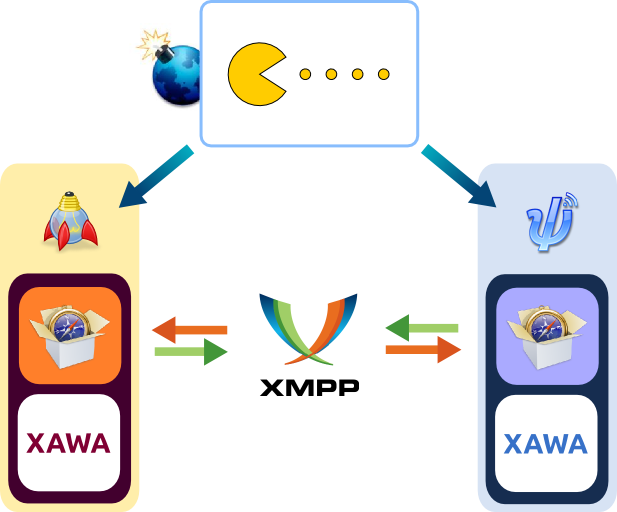
\includegraphics[width=80mm]{drawing.png}
	\end{center}
\end{frame}

%\section{Popis API}

\begin{frame}[fragile]


	\textbf{Textová komunikace:}

	\begin{lstlisting}[language=Javascript]
		xawa.sendMessage("ahoj!");
		
		var result = xawa.getMessage();
	\end{lstlisting}
	
	\vspace{5mm}
	
	\textbf{Datová komunikace:}
	
	\begin{lstlisting}[language=Javascript]
		xawa.sendData({
   pokusnyObject:[{
       id:1,
       text:"Lorem ipsum dolor"
   }]
		});
		
		var result = xawa.getData();
	\end{lstlisting}
\end{frame}

\begin{frame}

	\textbf{Co je zatím implementováno}
	\begin{itemize}
		\item základní plugin pro Jabbim
		\item textová komunikace
		\item datová komunikace
		\item jednoduché ukázkové aplikace
	\end{itemize}
	
	\vspace{5mm}
	
	\textbf{Co je ještě v plánu}
	\begin{itemize}
		\item změna formátu XMPP zpráv
		\item plugin pro Psi
		\item využití možností MUC
		\item port nějaké již existující aplikace
	\end{itemize}

\end{frame}

\begin{frame}
	\begin{center}
	\textbf{\LARGE{Děkuji za pozornost}}
	
	\vspace{5mm}
	\textbf{Dotazy?}
	\end{center}
\end{frame}


%\section{Struktura aplikací}

\begin{comment}

\begin{frame}{Popis API}
	\begin{itemize}
		\item gettery \textit{(getData(),...)}
		\item settery 
		\item metody pro komunikaci \textit{(sendMessage(),...)}
		\item speciální metody \textit{(init(),...)}
	\end{itemize}
\end{frame}


\begin{frame}[fragile]{Inicializace aplikace}

%	\begin{block}
		\begin{lstlisting}[language=HTML]
...
<script type="text/javascript">
		\end{lstlisting}
		\begin{lstlisting}[language=JavaScript]
  function appInit() {
    try {
      xawa.init();
      ...
    } catch(err) {
      // xawa init error handling
    }
  }
  		\end{lstlisting}
		\begin{lstlisting}[language=HTML]  	
</script>
...
<body onLoad="appInit();">
...
		\end{lstlisting}
%	\end{block}

\end{frame}

\begin{frame}[fragile]{Odesílání dat}
Odesílání textové zprávy
	\begin{lstlisting}[language=JavaScript]
xawa.sendMessage(message);	
	\end{lstlisting}
	
Odesílání dat (JSON)
	\begin{lstlisting}[language=JavaScript]
xawa.sendData(data);
	\end{lstlisting}
\end{frame}

\begin{frame}[fragile]{Příjem dat}

	\begin{lstlisting}[language=JavaScript]
...
xawa.init();
setInterval("getData()",1);
setInterval("getMessage()",1);
...		

function getData() {
  try {
    if (xawa.isUnread()) {
      var result = xawa.getData();
      // processing data
      ...
    }
  } catch (err) {
    // error handling
  }
}
	\end{lstlisting}
	
\end{frame}

\end{comment}

\end{document};
